
\section{Measurement details}
\label{sec:implementation}

\paragraph{Repeatability.} With fitness scores held fixed, one- and eight-device
Qwen2.5-0.5B updates agree to $6.3\times10^{-6}$ relative error in the norm of the whole parameter tree on the A100. The committed log reports this aggregate; it does not bound every leaf. Two
20-generation runs of the same eight-device program agree byte for byte. Separately
compiled programs need not follow the same training trajectory: changes in floating-point
arithmetic can change the selected token when greedy-decoding logits are nearly tied.

\subsection{The cost of ranking}
\label{sec:barrier}

Centered ranks require the scores of all candidates. Each device gathers and sorts
the same list. In an isolated v5e benchmark over 84 configurations, the ranking step
takes at most 60\,$\mu$s for populations up to a thousand and about 0.2\,ms at 4096.
At $N=2^{18}$, sorting takes 12.1\,ms and does not become faster with more devices,
because every device repeats it. Going from one to eight devices adds 9--10\,$\mu$s
at populations up to a thousand and 38.5\,$\mu$s at $N=2^{18}$. The isolated 1\,MiB score gather costs about 20\,$\mu$s, accounting for roughly half of the latter increase.
In full generations, turning score shaping on adds 41\,$\mu$s at $d=512$, $N=1024$
and 149\,$\mu$s at $d=2048$, $N=256$, within the repeat spread. Very large populations
should therefore budget for sorting even when gathering the scores is cheap.

\subsection{How the timing components are measured}
\label{sec:timemodel}

% generated by experiments/phase2/tb8.py; do not edit by hand
\begin{table}[t]
\centering
\small
\setlength{\tabcolsep}{4pt}
\caption{What one more collective costs inside a running program ($\mu$s; the slope of a dependent chain), $D{=}8$. The rows are what the placements issue: B's all-reduce of the $4P$-byte update and the $4N$-byte fitness gather. A program holding only the collective also pays a one-op floor (0.32\,ms on the A100, 0.60\,ms on the v5e) that a generation pays once. $\beta$ is payload over time.}
\label{tab:tb8}
\begin{tabular}{llrr}
\toprule
collective & payload & A100 & v5e \\
\midrule
all-reduce, latency floor & 8\,B & 27.2 & 5.7 \\
all-reduce (B), $d{=}512$ & 6\,MiB & 117.3 & 122.5 \\
all-reduce (B), $d{=}2048$ & 96\,MiB & 925.2 & 2006.0 \\
fitness gather, $N{=}256$ & 1\,KiB & 8.1 & 3.8 \\
fitness gather, $N{=}1024$ & 4\,KiB & 8.0 & 5.0 \\
fitness gather, $N{=}262144$ & 1\,MiB & 20.7 & 19.8 \\
\midrule
$\alpha$ ($\mu$s) & & 27 & 6 \\
$\beta$ (GiB/s) & & 98 & 47 \\
\bottomrule
\end{tabular}
\end{table}


Table~\ref{tab:tb8} uses a communication-only probe with a dependent chain of operations.
The increase in run time per additional operation estimates the collective's marginal
cost, excluding the fixed launch and synchronization cost of the compiled call. That
fixed cost is 0.32\,ms on the A100 and 0.60\,ms on the v5e. These are isolated
communication measurements, not timings extracted from a training trace.

\texttt{contraction\_isolation.py} similarly times three reconstruction probes: the
replicated path, the split path with its all-reduce, and the local split computation
with the all-reduce removed. The last two give $C_B$ and an estimate of the added cost
of communication. That difference can include scheduling changes caused by the
collective. It is not a directly isolated kernel duration.

The recorded replicated-probe slope includes A's gather of rank-derived weights.
\texttt{timemodel.py} subtracts the separately measured gather to obtain $C_A$ before
applying Eq.~\ref{eq:crossover}, so the gather is counted once.

Small reconstruction computations do not split ideally. On the A100,
$C_A/(D C_B)$ is 0.60--1.01 for full-rank noise and 0.18--0.45 for rank 1.
At width 2048, adding the all-reduce to the low-rank reconstruction probe costs
1.75--1.80 times the isolated communication benchmark on the A100, and 1.18--1.19 times
on the v5e. With measured local computation
and this added cost, the median absolute timing-model discrepancy is 0.63\,ms on the
A100 and 0.48\,ms on the v5e. The faster placement is identified in 18 of 20 and 15
of 16 configurations respectively; the three disagreements have measured gaps of
0.02--0.09\,ms. Correctly identifying a preference does not imply an accurate estimate
of its size: the largest discrepancies are 9.19\,ms on the A100 and 25.22\,ms on the
v5e. \texttt{timemodel.py} reports every configuration.

The measured-components model agrees with all 18 resolved A100 and all 12 resolved v5e
comparisons. The counts differ between platforms because the mirrored full-rank variant
was run only on A100. Replacing $C_B$ by $C_A/D$ and using the isolated collective
benchmark gives 17/20 and 16/16 sign agreements, including two resolved A100 misses:
mirrored rank 1 at $(d,N)=(512,256)$ and unpaired rank 1 at $(2048,256)$. For A100
low-rank noise at width 2048, this simple model predicts $t_A-t_B$ between $-0.49$
and $+0.18$\,ms, against $-1.63$ to $-0.84$\,ms measured. Keeping ideal splitting but
using the communication added to the reconstruction probe improves the counts to 19/20
and 16/16. Thus measured local reconstruction does not improve every near-tie; the added
communication cost is the important refinement for the resolved A100 cases.
\texttt{paper\_evidence.py} reproduces these comparisons and Table~\ref{tab:worked}.

\paragraph{What was fixed before measuring.} Before the single-host sweeps we expected
splitting to favor full-rank noise and replication to favor low-rank noise. The original
byte counts were subsequently corrected from compiled programs to include both score
and weight gathers. The timing equation was developed after these sweeps. It was used
prospectively at the host boundary, where the original prediction and the correction
below must be distinguished.

\subsection{Host-boundary prediction audit}
\label{sec:boundary-audit}

% generated by experiments/phase2/multihost/tb7_e18.py --latex; do not edit
\begin{table*}[t]
\centering
\small
\caption{Host-boundary prediction audit: split minus replicated time ($t_B-t_A$), in ms; negative favors splitting. Columns give hosts $\times$ devices per host. The original sixteen-device prediction used an overstated bandwidth; \emph{model} and \emph{corrected} use the actual calibration payload and were computed after the runs. Effective cross-host all-reduce bandwidth was 0.82\,GiB/s at eight devices and 0.58\,GiB/s at sixteen devices. The model starts from the earlier single-host sweep; the measured \texttt{1x8} column is a new measurement on the cluster's first host.}
\label{tab:tb7-audit}
\begin{tabular}{llrrrrrrr}
\toprule
 & & & & \multicolumn{2}{c}{\texttt{2x4}} & \multicolumn{3}{c}{\texttt{2x8}} \\
\cmidrule(lr){5-6}\cmidrule(lr){7-9}
variant & $d$ & $N$ & \texttt{1x8} & measured & model & measured & original & corrected \\
\midrule
seed & 2048 & 128 & $-21.4$ & $+86.8$ & $+91.0$ & $+74.1$ & $-13.9$ & $+137.2$ \\
seed & 2048 & 256 & $-50.8$ & $+57.2$ & $+58.7$ & $+56.7$ & $-48.2$ & $+103.0$ \\
seed & 512 & 1024 & $-20.1$ & $-13.0$ & $-18.9$ & $-24.8$ & $-27.0$ & $-17.6$ \\
rank 1 & 2048 & 128 & $+1.6$ & $+108.9$ & $+114.6$ & $+159.1$ & $+11.7$ & $+162.7$ \\
rank 1 & 2048 & 256 & $+1.4$ & $+111.4$ & $+114.4$ & $+130.9$ & $+11.4$ & $+162.5$ \\
rank 1 & 512 & 1024 & $0.0$ & $+6.9$ & $+7.1$ & $+7.8$ & $+0.8$ & $+10.2$ \\
\bottomrule
\end{tabular}
\end{table*}


The calibration used for the sixteen-device prediction all-reduced $1/D$ of its labelled
payload, overstating bandwidth by a factor of $D$. This was discovered after the runs.
Table~\ref{tab:tb7-audit} retains the prediction made with that calibration and the
retrospective correction at the actual payload size. The latter identifies all six
preferences, but overestimates the split penalty by up to 63\,ms. The calibration
and isolated ladder use different payloads and timing methods; their bandwidth numbers
are not evidence of a difference between hardware sessions.

For the fixed-eight-device comparison, let $S=t_A-t_B$ be the within-host saving and
$T_{\mathrm{intra}}$ the communication being replaced. Neglecting latency and holding
reconstruction costs fixed, the cross-host break-even rate is
$\beta_*=4P/(S+T_{\mathrm{intra}})$. At width 2048, $S$ is 21.4 or 50.8\,ms at
$N=128$ or 256; the within-host bandwidth term at 96\,MiB is 1.46\,ms. This gives
4.1 and 1.8\,GiB/s. Using repeat extremes gives 2.9--4.2 and 1.5--2.1\,GiB/s.
These are approximate effective collective rates, including algorithmic traffic in the
measured bandwidth, not line rates. The earlier sixteen-device prediction had the same
ordering, with thresholds of 4.12 and 1.70\,GB/s (decimal units); it also assumed extra
compute savings from using sixteen devices. The two calculations are not identical tests.

\paragraph{Other placements and overlap.} The two placements are not exhaustive.
One primary device can reconstruct the whole update and broadcast the model, as in
EGGROLL's vLLM setup \citep[Appendix L.2]{eggroll2025}. It avoids repeated reconstruction
across replicas, but retains a full reconstruction on the critical path and adds a
model-sized broadcast. We did not benchmark this third placement. Under an otherwise
identical synchronous cost model it adds communication to A; heterogeneous devices,
memory limits and implementation differences could change the comparison. Hierarchical
or compressed communication also changes the tradeoff; PowerSGD communicates low-rank
approximations of updates rather than the dense arrays studied here \citep{vogels2019}.
Overlapping an update's all-reduce with the next generation's evaluation would use stale
weights. Within a generation, bucketing partial updates could overlap local reconstruction with
communication, as in distributed backpropagation \citep{li2020ddp}. Such overlap can
at best replace $C_B+T_{\mathrm{ar}}$ by $\max(C_B,T_{\mathrm{ar}})$ under the
accounting model. With the measured probe costs, replication retains a 0.40--1.98\,ms
lead at every low-rank width-2048 configuration. This is a conditional bound from
\texttt{overlap\_bound.py}, not an implemented overlap experiment.



\subsection{What model size alone can predict}
\label{sec:size}

A conditional scaling argument helps separate parameter count from implementation
constants. Suppose the leading low-rank reconstruction cost is $C_A=kPNr$, with $k$ absorbing
pairing and arithmetic efficiency, and $C_B=qC_A$. Write the collective time
as $\alpha+4P/\beta$. Equation~\ref{eq:crossover} then favors splitting when
\[
  (1-q)kNr > \frac{4}{\beta}
               +\frac{\alpha-T_{\mathrm{ag}}(4N)}{P}.
\]
For bandwidth-dominated communication, fixed $k,q,\beta$ and large $P$, the leading
parameter-count dependence cancels. Population times rank, rather than parameter count
alone, then sets the balance. For full-rank noise, the analogous assumption is
$C_A=kPN$. These assumptions are not automatic: matrix shapes and compiler fusion change
$k$, small local computations change $q$, and the collective rate depends on message size
and topology. Factor generation also has terms proportional to $Nr(m+n)$ rather than
$P$. We therefore do not turn the block's constants into a universal threshold or a
claim about 7B models. Such a model would need to fit on each device, and its
reconstruction and collective costs would need measurement.

\section{Cost and implementation comparisons}
\label{sec:systems-ablations}
\label{sec:refimpl}

\begin{figure*}[t]
  \centering
  
\includegraphics[width=\textwidth]{f4-cost-bfloat16.png}
  \caption{The full single-device cost and feasibility grid, relative to stored
    full-rank noise at each model width and population. Blue is faster, red slower.
    Hatched cells mean the dense baseline does not fit; blank cells marked ``both OOM''
    mean neither variant fits. Memory feasibility is separate from a measured speedup.
    The main text compares only configurations feasible on both platforms.}
  \label{fig:f4-full}
\end{figure*}

% generated by experiments/phase2/tb3.py; do not edit by hand
\begin{table*}
\centering
\small
\caption{Systems ablations, assembled from committed results. Each ratio is the time of the first variant over the second (below one: the first is faster), as a geometric mean over the configurations where both were measured (n: how many).}
\label{tab:tb3}
\begin{tabular}{p{0.30\linewidth}p{0.22\linewidth}p{0.40\linewidth}}
\toprule
ablation & where & result \\
\midrule
cost, rank 1 vs dense & A100, bf16 & 0.22x (n=9) \\
cost, rank 4 vs dense & A100, bf16 & 0.27x (n=9) \\
cost, rank 16 vs dense & A100, bf16 & 0.29x (n=9) \\
cost, rank 1 vs dense & TPU v5e, bf16 & 0.08x (n=7) \\
cost, rank 4 vs dense & TPU v5e, bf16 & 0.09x (n=7) \\
cost, rank 16 vs dense & TPU v5e, bf16 & 0.11x (n=7) \\
cost, bf16 vs f32 & A100, dense & 1.12x (n=8) \\
cost, bf16 vs f32 & A100, seed & 1.08x (n=20) \\
cost, bf16 vs f32 & A100, rank 1 & 1.00x (n=14) \\
cost, bf16 vs f32 & TPU v5e, dense & 0.93x (n=6) \\
cost, bf16 vs f32 & TPU v5e, seed & 1.01x (n=20) \\
cost, bf16 vs f32 & TPU v5e, rank 1 & 0.97x (n=16) \\
cost, highest vs default & TPU v5e, dense & 1.08x (n=5) \\
cost, highest vs default & TPU v5e, rank 1 & 1.85x (n=6) \\
cost, highest vs default & TPU v5e, rank 16 & 1.64x (n=6) \\
cost, highest vs default & TPU v5e, rank 4 & 1.76x (n=6) \\
cost, highest vs default & TPU v5e, seed, mirrored & 1.02x (n=6) \\
cost, highest vs default & TPU v5e, seed & 1.02x (n=6) \\
\bottomrule
\end{tabular}
\end{table*}


Figure~\ref{fig:f4-full} includes the configurations excluded from the common-grid speed
comparison because one or more variants do not fit. Table~\ref{tab:tb3} separates three
choices: perturbation rank, storage datatype, and matrix-multiplication precision.
The precision setting controls internal multiplication accuracy, separately from array
storage. On the v5e, forcing JAX's highest precision instead of its default costs the
low-rank variants 1.6--1.9 times in run time and the full-rank variants at most 8\%.
Its effect on learning accuracy was not measured. Default precision reduces low-rank
reconstruction cost further, which, with communication fixed, favors replication in
Eq.~\ref{eq:crossover}; the placement sweeps nevertheless keep highest precision fixed. Storage datatype alone changes the
reported geometric-mean times by much less; it should not be confused with this
precision setting.

% generated by experiments/phase2/tb1.py; do not edit by hand
\begin{table*}[t]
\centering
\small
\setlength{\tabcolsep}{5pt}
\caption{Throughput at matched shapes: token-position evaluations per second (tokens = population $\times$ batch $\times$ sequence). \emph{rank 1} and \emph{seed} are this library's variants; \emph{EGGROLL} is its authors' released code; \emph{naive} gives every member its own copy of the weights, evaluating the population in parallel; \emph{evosax} is OpenES in the incumbent JAX library. None of the three references shards, so only the library's variants have a $D{=}8$ column. Seed evaluates one candidate at a time to keep weight memory at $O(P)$. Qiu et al.'s released code is not included. OOM: does not fit the device at this shape.}
\label{tab:tb1}
\begin{tabular}{llrrrrrrr}
\toprule
 & & \multicolumn{2}{c}{rank 1} & EGGROLL & \multicolumn{2}{c}{seed} & naive & evosax \\
\cmidrule(lr){3-4}\cmidrule(lr){6-7}
shape & platform & $D{=}1$ & $D{=}8$ & $D{=}1$ & $D{=}1$ & $D{=}8$ & $D{=}1$ & $D{=}1$ \\
\midrule
$d{=}512$, $N{=}256$ & A100 & 21.30M & 27.24M & 21.76M & 1.43M & 5.86M & 5.19M & 5.36M \\
$d{=}512$, $N{=}256$ & TPU v5e & 23.33M & 46.80M & 27.29M & 484k & 3.54M & 3.71M & 2.97M \\
$d{=}512$, $N{=}1024$ & A100 & 26.03M & 84.46M & 25.56M & 1.45M & 9.44M & 5.42M & 5.58M \\
$d{=}512$, $N{=}1024$ & TPU v5e & 16.77M & 149.67M & 24.72M & 486k & 3.81M & 3.74M & 2.33M \\
$d{=}2048$, $N{=}128$ & A100 & 2.97M & 6.79M & 3.05M & 314k & 1.87M & 406k & 375k \\
$d{=}2048$, $N{=}128$ & TPU v5e & 3.35M & 7.02M & 4.15M & 34k & 266k & 204k & OOM \\
$d{=}2048$, $N{=}256$ & A100 & 3.20M & 10.88M & 3.21M & 315k & 2.06M & 409k & 377k \\
$d{=}2048$, $N{=}256$ & TPU v5e & 3.22M & 13.03M & 4.52M & 34k & 270k & 140k & OOM \\
\bottomrule
\end{tabular}
\end{table*}


\paragraph{Matched-device comparison.} Table~\ref{tab:tb1} compares released
implementations at the same block configurations. The naive baseline gives each
candidate a separate copy of the model; evosax uses OpenES. At one device, the library's
rank-1 throughput is 0.97--1.02 times EGGROLL's on the A100 and 0.68--0.85 times on
the v5e. The TPU difference was not isolated. We did not benchmark Qiu et al.'s released
implementation, so the seed column is not a timing of their code.

\paragraph{Additional devices.} The tested reference implementations do not split the
population across devices. The eight-device columns therefore show extra throughput
from extra hardware, not equal-resource speedups over those references. Compared with
one-device EGGROLL, the library on eight devices reaches 1.3--3.4 times the throughput on A100
and 1.7--6.1 times on v5e. The full scaling grids report each implementation path against
its own smallest device count.

\paragraph{Implementation boundaries.} EGGROLL's reference rank-1 path does not compile
on a 16\,GB TPU chip at $d=512$, $N=16384$: it requests 24.1\,GiB of temporaries.
The library avoids this compiler behavior by padding rank-1 factors with a zero column
on TPU, retaining a fused multiply; it runs that configuration in 245\,ms. The GPU
compiler does not need the padding. The tested reference also declines embedding tables,
which the library supports through the same interface as matrix layers. These are properties
of the tested code versions, not limitations of the algorithms.


\section{Real-model timing and memory}
\label{sec:memory}

% generated by experiments/countdown/tb5_e17.py --latex; do not edit
\begin{table*}[t]
\centering
\small
\caption{What one real-model update costs, in ms (Qwen2.5-0.5B, one ask, next-token loss and tell on the fixed prompt batch, TPU v5e-8, median of five repeats). Each entry is the faster of the two placements; Figure~\ref{fig:f9} gives the ratio between them. OOM: neither placement fits a 16\,GB chip at that shape.}
\label{tab:tb5}
\begin{tabular}{llrrrr}
\toprule
arm & $N$ & $D{=}1$ & $D{=}2$ & $D{=}4$ & $D{=}8$ \\
\midrule
seed, mirrored & 32 & 4902 & 2481 & 1263 & 673 \\
seed, mirrored & 64 & 9788 & 4893 & 2469 & 1276 \\
seed, mirrored & 128 & 19559 & 9718 & 4882 & 2482 \\
seed, mirrored & 240 & 36658 & 18159 & 9102 & 4590 \\
rank 1 & 32 & OOM & 217 & 109 & 71 \\
rank 1 & 64 & OOM & OOM & 219 & 122 \\
rank 1 & 128 & OOM & OOM & OOM & 230 \\
rank 1 & 240 & OOM & OOM & OOM & OOM \\
rank 4 & 32 & OOM & 211 & 111 & 72 \\
rank 4 & 64 & OOM & OOM & 214 & 119 \\
rank 4 & 128 & OOM & OOM & OOM & 227 \\
rank 4 & 240 & OOM & OOM & OOM & OOM \\
rank 16 & 32 & OOM & 225 & 117 & 78 \\
rank 16 & 64 & OOM & OOM & 241 & 136 \\
rank 16 & 128 & OOM & OOM & OOM & 272 \\
rank 16 & 240 & OOM & OOM & OOM & OOM \\
\bottomrule
\end{tabular}
\end{table*}


Table~\ref{tab:tb5} gives absolute generation times behind Figure~\ref{fig:f9}.
The original grid has 128 records; 63 carry a dirty-worktree flag. Historical launch
scripts ran other probes first, which could dirty result files, but no per-run diff
was saved to certify that only outputs changed. We therefore exclude those records.
The remaining 65 include 43 timings and 22 memory failures; only configurations with
two clean records enter a placement comparison. This leaves twelve low-rank and eight
full-rank timing comparisons. All eight-device records are clean. Excluded comparisons
are dashes, distinct from observed memory failures; historical records remain available
for audit in the experiment directory.

At eight devices, ranks 1, 4 and 16 fit populations up to 128 and all fail at 240; the
regenerated full-rank variant fits all four populations. The evaluation schedules differ:
full rank scans individual candidates, while low rank batches them with a shared base
weight matrix. A diagnostic CPU compilation probe on a reduced model finds temporary
memory growing with candidates and prompts when candidates are batched. Batching
full-rank evaluation in the same way reproduces that growth, rather than the flat
population dependence of scanning. This supports an activation-memory explanation,
but is not a measured matched-batching memory boundary for Qwen on TPU.

\section{Synthetic alignment}
\label{sec:alignment}

% generated by experiments/countdown/tb6_e16.py --latex; do not edit
\begin{table*}[t]
\centering
\small
\caption{Alignment measurements and prediction audit ($\times10^{-4}$; median [min, max] across five seeds). \emph{Later reference} uses the full-rank synthetic fit at $N/P$, selected after the runs. \emph{Original prediction} was fixed before each run and uses the variant's fit at $N/d_{\mathrm{samp}}$ (with the advance correction at 1.5B described in the text). Ratios are measured / predicted.}
\label{tab:tb6-audit}
\begin{tabular}{lllrrrrr}
\toprule
 & & & & \multicolumn{2}{c}{later reference} & \multicolumn{2}{c}{original prediction} \\
\cmidrule(lr){5-6}\cmidrule(lr){7-8}
model & arm & $N$ & measured & pred. & ratio & pred. & ratio \\
\midrule
0.5B & seed, mirrored & 30 & $1.42$ [1.3, 1.9] & $1.56$ & $0.91$ & $1.56$ & $0.91$ \\
0.5B & seed, mirrored & 240 & $4.23$ [3.8, 4.4] & $4.48$ & $0.94$ & $4.48$ & $0.94$ \\
0.5B & rank 1 & 30 & $1.37$ [1.2, 1.7] & $1.56$ & $0.88$ & $2.69$ & $0.51$ \\
0.5B & rank 1 & 240 & $3.91$ [3.8, 4.2] & $4.48$ & $0.87$ & $7.57$ & $0.52$ \\
0.5B & rank 4 & 30 & $1.87$ [0.7, 2.0] & $1.56$ & $1.20$ & $2.78$ & $0.67$ \\
0.5B & rank 4 & 240 & $4.42$ [4.1, 4.8] & $4.48$ & $0.99$ & $7.85$ & $0.56$ \\
0.5B & rank 16 & 30 & $1.49$ [1.1, 1.7] & $1.56$ & $0.95$ & -- & -- \\
0.5B & rank 16 & 240 & $4.09$ [3.9, 4.5] & $4.48$ & $0.91$ & -- & -- \\
0.5B & rank 1, unpaired & 30 & $1.60$ [1.1, 1.9] & $1.56$ & $1.03$ & $3.76$ & $0.43$ \\
0.5B & rank 1, unpaired & 240 & $5.33$ [5.1, 5.5] & $4.48$ & $1.19$ & $10.56$ & $0.50$ \\
\midrule
0.5B, second batch & seed, mirrored & 240 & $4.20$ [3.8, 4.4] & $4.48$ & $0.94$ & $4.48$ & $0.94$ \\
0.5B, second batch & rank 1 & 240 & $3.91$ [3.8, 4.2] & $4.48$ & $0.87$ & $7.57$ & $0.52$ \\
\midrule
1.5B & seed, mirrored & 30 & $0.83$ [0.8, 0.9] & $0.87$ & $0.95$ & $0.87$ & $0.95$ \\
1.5B & seed, mirrored & 240 & $2.32$ [2.0, 2.6] & $2.51$ & $0.92$ & $2.51$ & $0.92$ \\
1.5B & rank 1 & 30 & $0.77$ [0.4, 1.1] & $0.87$ & $0.89$ & $1.04$ & $0.74$ \\
1.5B & rank 1 & 240 & $2.27$ [1.9, 2.4] & $2.51$ & $0.91$ & $2.93$ & $0.77$ \\
\bottomrule
\end{tabular}
\end{table*}




% F5 -- experiments/phase0/figures/f5-estimator-quality.png (experiments/phase0/plot.py)
\begin{figure}[t]
  \centering
  
\includegraphics[width=\linewidth]{f5-estimator-quality.png}
  \caption{Alignment on the synthetic block ($\sigma{=}10^{-3}$, centered ranks):
    $\cos(\Delta\theta, -\nabla L)$ for the squared-error loss, against $N/P$, median and
    interquartile band over 30 replicates. The three ranks lie on top of each other.
    Dotted: the Gaussian-projection approximation, unpaired and mirrored.}
  \label{fig:f5}
\end{figure}

\paragraph{The Gaussian-projection approximation.} Let $z_i$ be member $i$'s
perturbation projected onto the unit descent direction, $\langle\epsilon_i, -\nabla
L\rangle/\lVert\nabla L\rVert$. It has unit variance for full-rank and for low-rank
noise, since $UV^\top/\sqrt r$ has identity covariance. If the loss is locally linear,
ranking the members by loss ranks them by $z_i$, and if $z_i$ is Gaussian each
$\epsilon_i$ enters Eq.~\ref{eq:update} with a coefficient close to $\Phi(z_i)-\tfrac12$
for large $N$. The update's component along the
descent direction is then about $N\,\mathbb{E}[(\Phi(z)-\tfrac12)\,z] = N/(2\sqrt\pi)$
and, for $N\ll P$, its norm is about $\sqrt{NP\,\mathbb{E}[(\Phi(z)-\tfrac12)^2]} =
\sqrt{NP/12}$, so the cosine is $\sqrt{3/\pi}\,\sqrt{N/P}$. A mirrored pair contributes
one direction with twice the weight, and $N/2$ of them give $1/\sqrt2$ of that.

\paragraph{When the projection is Gaussian.} For full-rank Gaussian noise $z_i$ is
exactly Gaussian. For rank-$r$ noise on a matrix with gradient $G$, the projection is a
sum over the $r$ factor pairs of $a^\top G b$, summed again over matrices. If $G$ has
rank one, $G = uv^\top$, each term is $(a^\top u)(v^\top b)$, a product of two Gaussians,
however many entries of $G$ are nonzero. The projection approaches a Gaussian as the
gradient spreads over many singular directions and many matrices, and as $r$ grows. We
did not measure the gradient's spectrum on Qwen, so for the real model the approximation
is a scale estimate, not a derivation.

Figure~\ref{fig:f5} is the synthetic study behind Section~\ref{sec:quality}, one slice
of 456 configurations of 30 replicates each. Against $N/P$ the mirrored variants of every
rank coincide, the largest over the smallest at equal $N$ being 1.01--1.04, and every
variant is within 0.91--1.02 of the approximation; its log-log slopes are 0.494--0.508. Unpaired sampling lies 1.34--1.53$\times$ above mirrored, about $\sqrt2$.
Orthogonal (Hadamard) and scrambled Sobol sampling, not drawn, are within 0.97--1.04 of
plain mirroring. That null result holds for this high-dimensional, small-population
regime; it is not a claim about coupled sampling in general.

The predictions frozen before the real-model runs used $N/d_{\mathrm{samp}}$ instead,
where $d_{\mathrm{samp}}$ is the number of independent random numbers in one
perturbation: the parameter count for full-rank noise and $r(m+n)$ per $m\times n$
matrix at rank $r$ (other parameters count fully). Each variant's own fit against that axis
was the prediction, and Table~\ref{tab:tb6-audit} keeps it next to the synthetic reference. Its extra 0.5B
prompt check reuses the same perturbation keys and changes only puzzle numbers within
the same prompt template. It measures sensitivity to that change, not an independent
replication; it is excluded from the main table. On the block, where every matrix is $512\times512$, $P/d_{\mathrm{samp}}$ is
256 at rank 1 and 64 at rank 4. On Qwen2.5 the matrices are larger and not square, and it
is 638 and 171 at 0.5B and 1063 and 287 at 1.5B, so the same $N$ sits further right on
the $N/d_{\mathrm{samp}}$ axis than on the block and the fitted curve predicts higher alignment. At a
slope of one half that overstates rank 1 by $\sqrt{638/256}\approx1.6$ and rank 4 by
$\sqrt{171/64}\approx1.6$ at 0.5B, against measured shortfalls of 1.9--2.0 and 1.5--1.8.
The same fits predicted full rank within 9\%, since $P/d_{\mathrm{samp}}$ is 1 for it on
every model. For rank 1 at 1.5B the prediction was multiplied by a correction of 0.53
measured at 0.5B and fixed in advance; the observations were still 23--26\% below it.


At equal population, unpaired rank 1 has 1.36 times the mirrored alignment at $N=240$
and 1.17 times at $N=30$ on the original 0.5B batch. The former is close to the
$\sqrt2$ ratio of the independent-direction approximation. This comparison is specific
to the tested loss and noise scale; it does not establish that unpaired sampling is
better for training. The theoretical approximation and the fitted synthetic reference
are also distinct: the latter is the reference column in Table~\ref{tab:tb6-audit}.


\section{Countdown details}
\label{sec:countdown}

\begin{table*}[t]
\centering
\small
\caption{Countdown training configuration. A sample evaluation is one scored \emph{training}
  completion (held-out scoring is not counted); every population-30 variant uses 240 per update (30
  members $\times$ 8 puzzles), so 120,000 is 500 updates.}
\label{tab:e2e}
\begin{tabular}{lp{0.76\linewidth}}
\toprule
task, reward & Countdown; 1.0 solved, 0.1 well formed but wrong, 0.0 otherwise \\
data & training pool of 256 puzzles, 8 per update; 2000 disjoint held-out puzzles \\
prompts, decoding & chat template, prompts padded to 128 tokens, 96 new tokens; greedy \\
variants & $N{=}30$, $\sigma{=}10^{-3}$, $\eta{=}5\times10^{-7}$ in Eq.~\ref{eq:update},
  centered ranks; seed, mirrored and ranks 1, 4, 16, plus rank 1 with the embedding (27\%
  of the parameters) frozen \\
budget, seeds & 120,000 sample evaluations per run; seeds 0--2 per variant \\
evaluation & 2000 held-out puzzles every 50 updates, before the first and after the last \\
hardware & one A100-SXM4-80GB; about 13\,h for the campaign \\
\bottomrule
\end{tabular}
\end{table*}

\paragraph{Relation to the published setup.} \citet{qiu2025} use
$\Delta\theta=\alpha\sum_i z_i\epsilon_i/N$ with $\alpha=5\times10^{-4}$ and
standardized rewards $z_i$. Taking $\eta=\alpha\sigma$ converts their learning-rate
convention to Eq.~\ref{eq:update}. Our centered ranks replace standardized rewards;
the nominal weight standard deviations are about 0.29 and 1, and we did not match the
resulting update magnitudes. Our batches contain eight puzzles per update rather than
200 samples. The experiment therefore compares our perturbation variants, not a
reproduction of the published learning curve.

\paragraph{Timing.} The time axis in Figure~\ref{fig:f7} excludes updates 0 and 1,
which compile (322--635\,s each), and all held-out decoding. These are material costs
for a short run; the axis is steady-state update time rather than total experiment time.
The displayed learning curves use the campaign with clean recorded provenance.
Diagnostic batching probes are not used as reported performance results.

\begin{figure}[t]
  \centering
  
\includegraphics[width=\linewidth]{f7-e13-frozen.png}
  \caption{Freezing the embedding changes which parameters can train. The frozen
    embedding accounts for 27\% of parameters; this rank-1 variant ends at a lower
    observed solve rate. Means and min--max bands over three seeds.}
  \label{fig:f7-frozen}
\end{figure}

\paragraph{Freezing the embedding.} This variant asks what leaving the tied embedding
out of training costs. It contains 27\% of the parameters, and the tested EGGROLL
reference declines it (Appendix~\ref{sec:refimpl}). The library can perturb it without
forming a full table per candidate. Freezing it gives 5.55\% mean final solve rate
[5.20, 6.00], against 6.18\% [6.10, 6.35] for rank 1 updating all parameters, with
non-overlapping seed ranges (Figure~\ref{fig:f7-frozen}). Thus embedding support has
value in this experiment, although this extra intervention is not a comparison of
perturbation ranks alone.

\begin{figure}[t]
  \centering
  
\includegraphics[width=\linewidth]{f7c-e19-n16.png}
  \caption{An additional population-size experiment: population 30 (solid, 500 updates)
    and 16 (dashed, 940 updates), with about 120,000 scored completions each and three
    seeds per variant. Population 16 approaches the plateau sooner per completion, but
    also receives more updates. This does not isolate per-update alignment.}
  \label{fig:f7c}
\end{figure}

\paragraph{The intended positive control.} The population-16 run was fixed in advance
as a control with 27\% lower predicted per-update alignment. At approximately the same
completion budget it takes 940 updates instead of 500 and reaches the plateau sooner
(Figure~\ref{fig:f7c}). Thus it does not establish that this task can distinguish small
differences in update quality. The final observed accuracy is similar.

\section{Scaling grids}
\label{sec:grids}

Figures~\ref{fig:m1-a100}--\ref{fig:m2-tpu} are the full strong- and weak-scaling grids,
every perturbation variant under both placements. Both show parallel efficiency, each series against its
own smallest measured device count, so the ideal is 1 for every series; the strong-scaling
figures add time per generation, and the weak-scaling figures peak memory per device. At $d{=}2048$ and 32 members per device the rank-1 variants keep
0.86--0.93 efficiency at eight devices on the A100 and 0.71--0.91 on the v5e. What
degrades is a placement: under replication the dense and seed variants fall to 0.39 and 0.50
on the A100 (0.18 and 0.54 on the v5e), because they have the most work to repeat, and
under all-reduce the same variants hold 0.79--1.00. The v5e grid has efficiencies above one,
all at $d{=}512$ (rank 1 at $N{=}1024$ reaches 1.22 at $D{=}2$): there the single chip is
memory-bound, and splitting the population relieves it. The dense variant with all-reduce has
no one-device point at $d{=}2048$, $N{=}256$ on the v5e (out of memory), so its efficiency
is normalized at $D{=}2$.

% M1/M2 per platform. Explicit paths: the A100 and TPU sets share filenames.
\begin{figure*}[p]
  \centering
  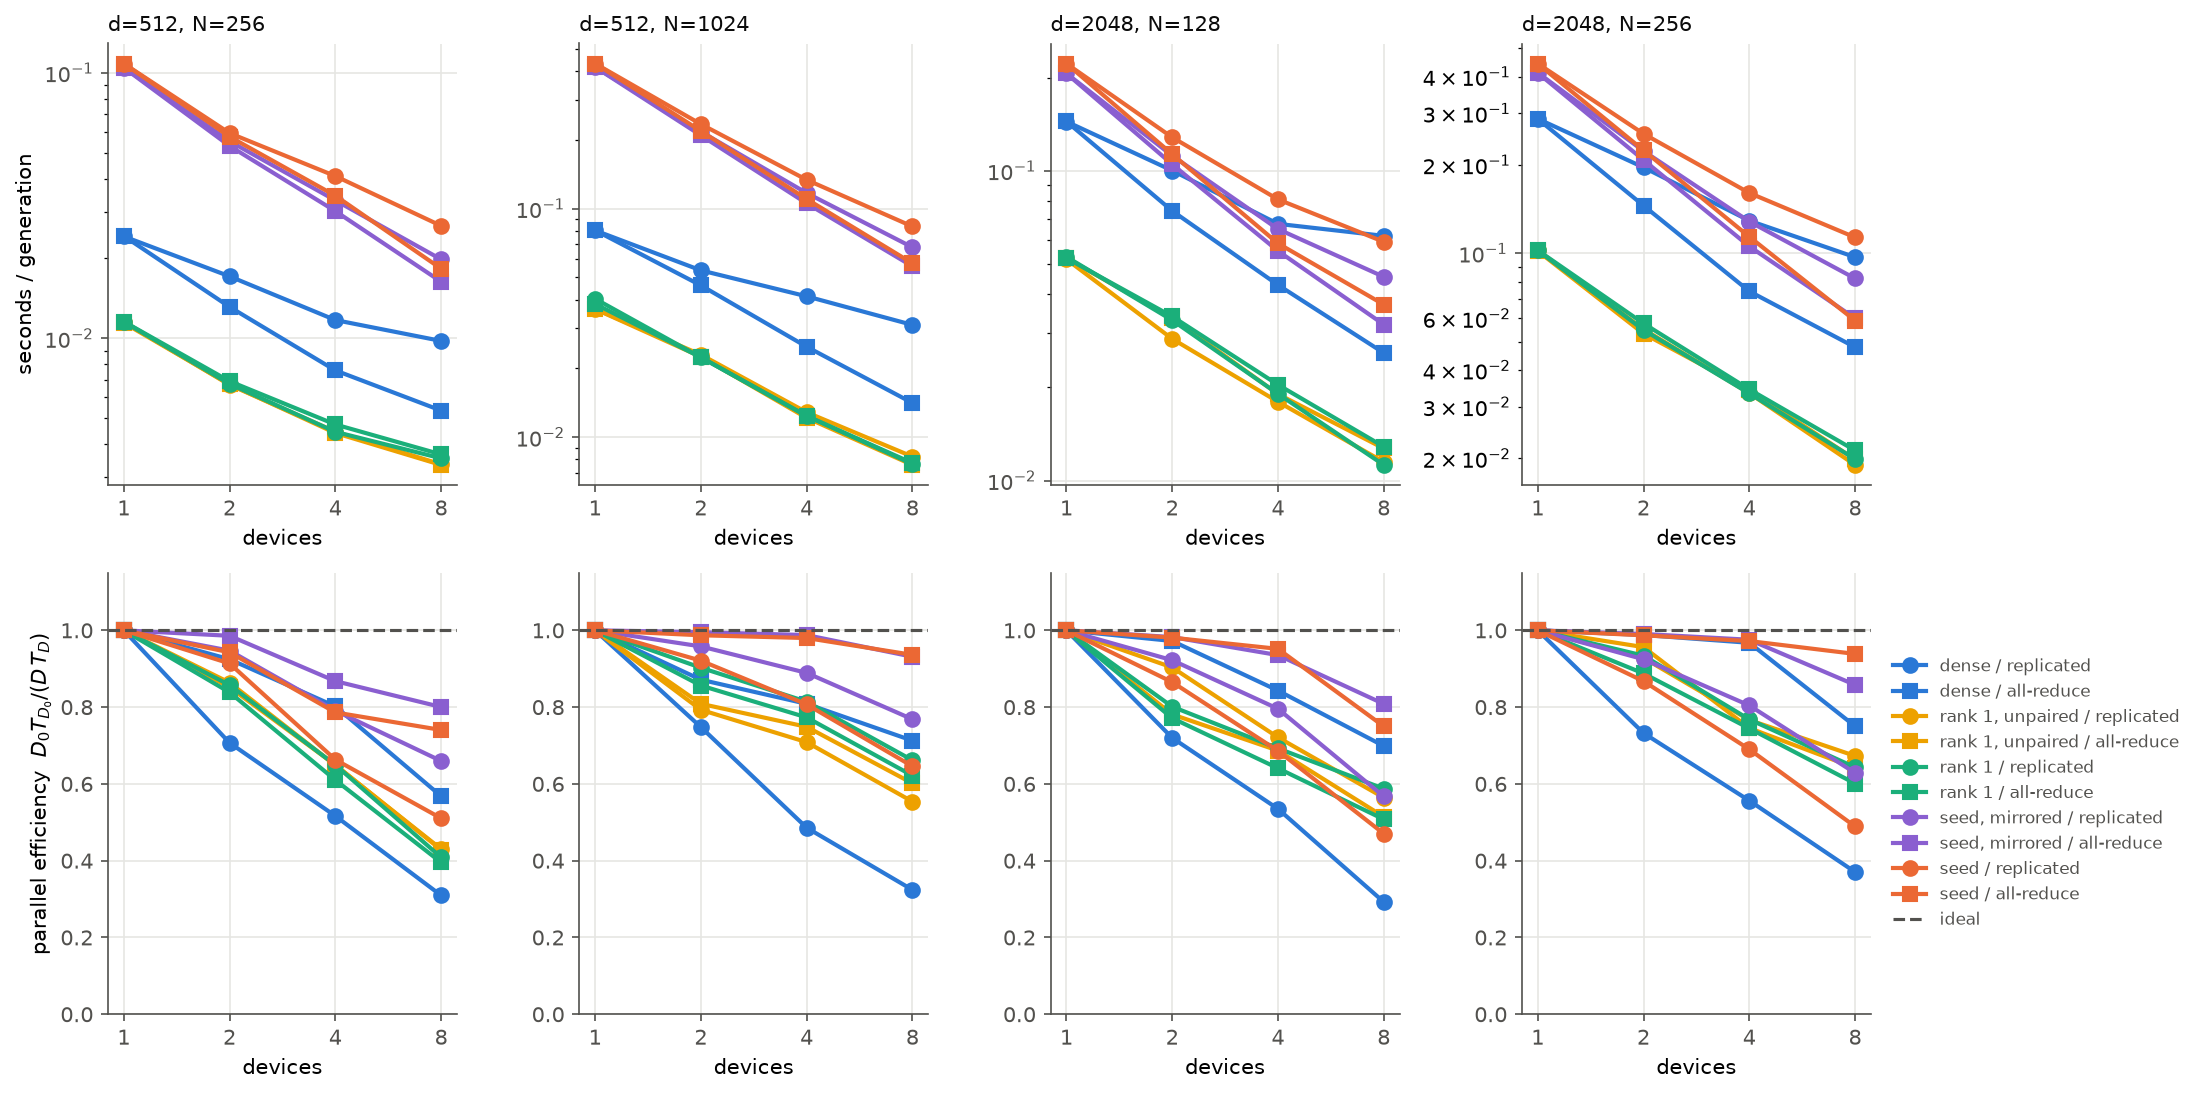
\includegraphics[width=.9\textwidth]{../experiments/phase2/figures/m1-strong-scaling.png}
  \caption{A100 strong scaling at fixed total population: generation time (top) and
    parallel efficiency (bottom), relative to each series' smallest device count.
    An efficiency of 1 means ideal scaling. Every perturbation variant is shown under
    both replicated and split update placement.}
  \label{fig:m1-a100}
\end{figure*}
\begin{figure*}[p]
  \centering
  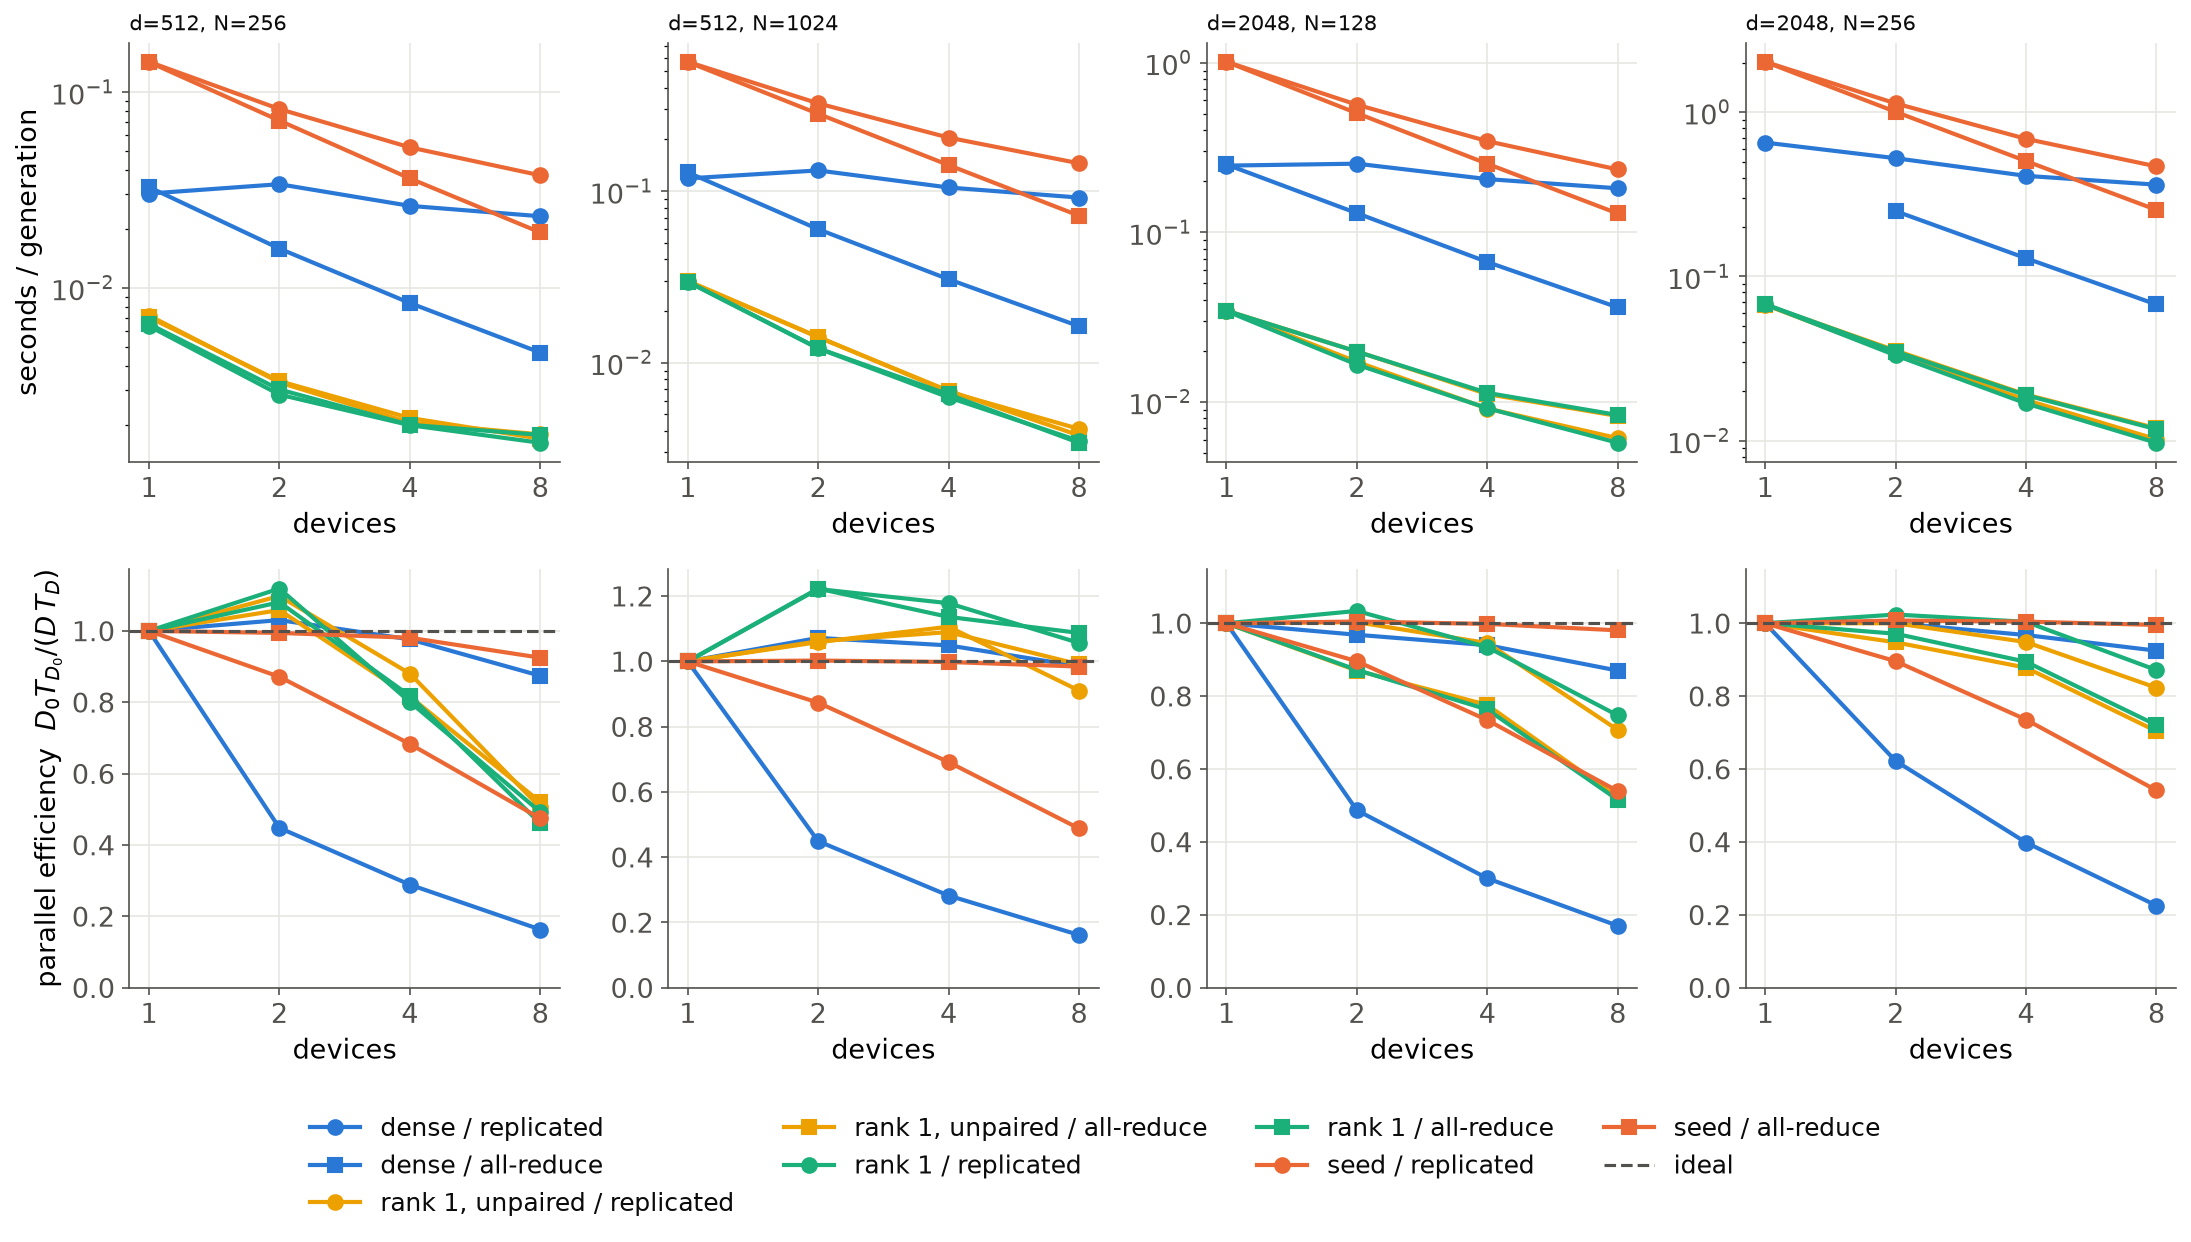
\includegraphics[width=.9\textwidth]{../experiments/phase2/figures-tpu-v5e8/m1-strong-scaling.png}
  \caption{TPU strong scaling at fixed total population: generation time (top) and
    efficiency (bottom). Dense noise with splitting at $d=2048$, $N=256$ is normalized
    at two devices because it does not fit on one. Some width-512 cases exceed unit
    efficiency when splitting the population relieves the single-device bottleneck.}
  \label{fig:m1-tpu}
\end{figure*}
\begin{figure*}[p]
  \centering
  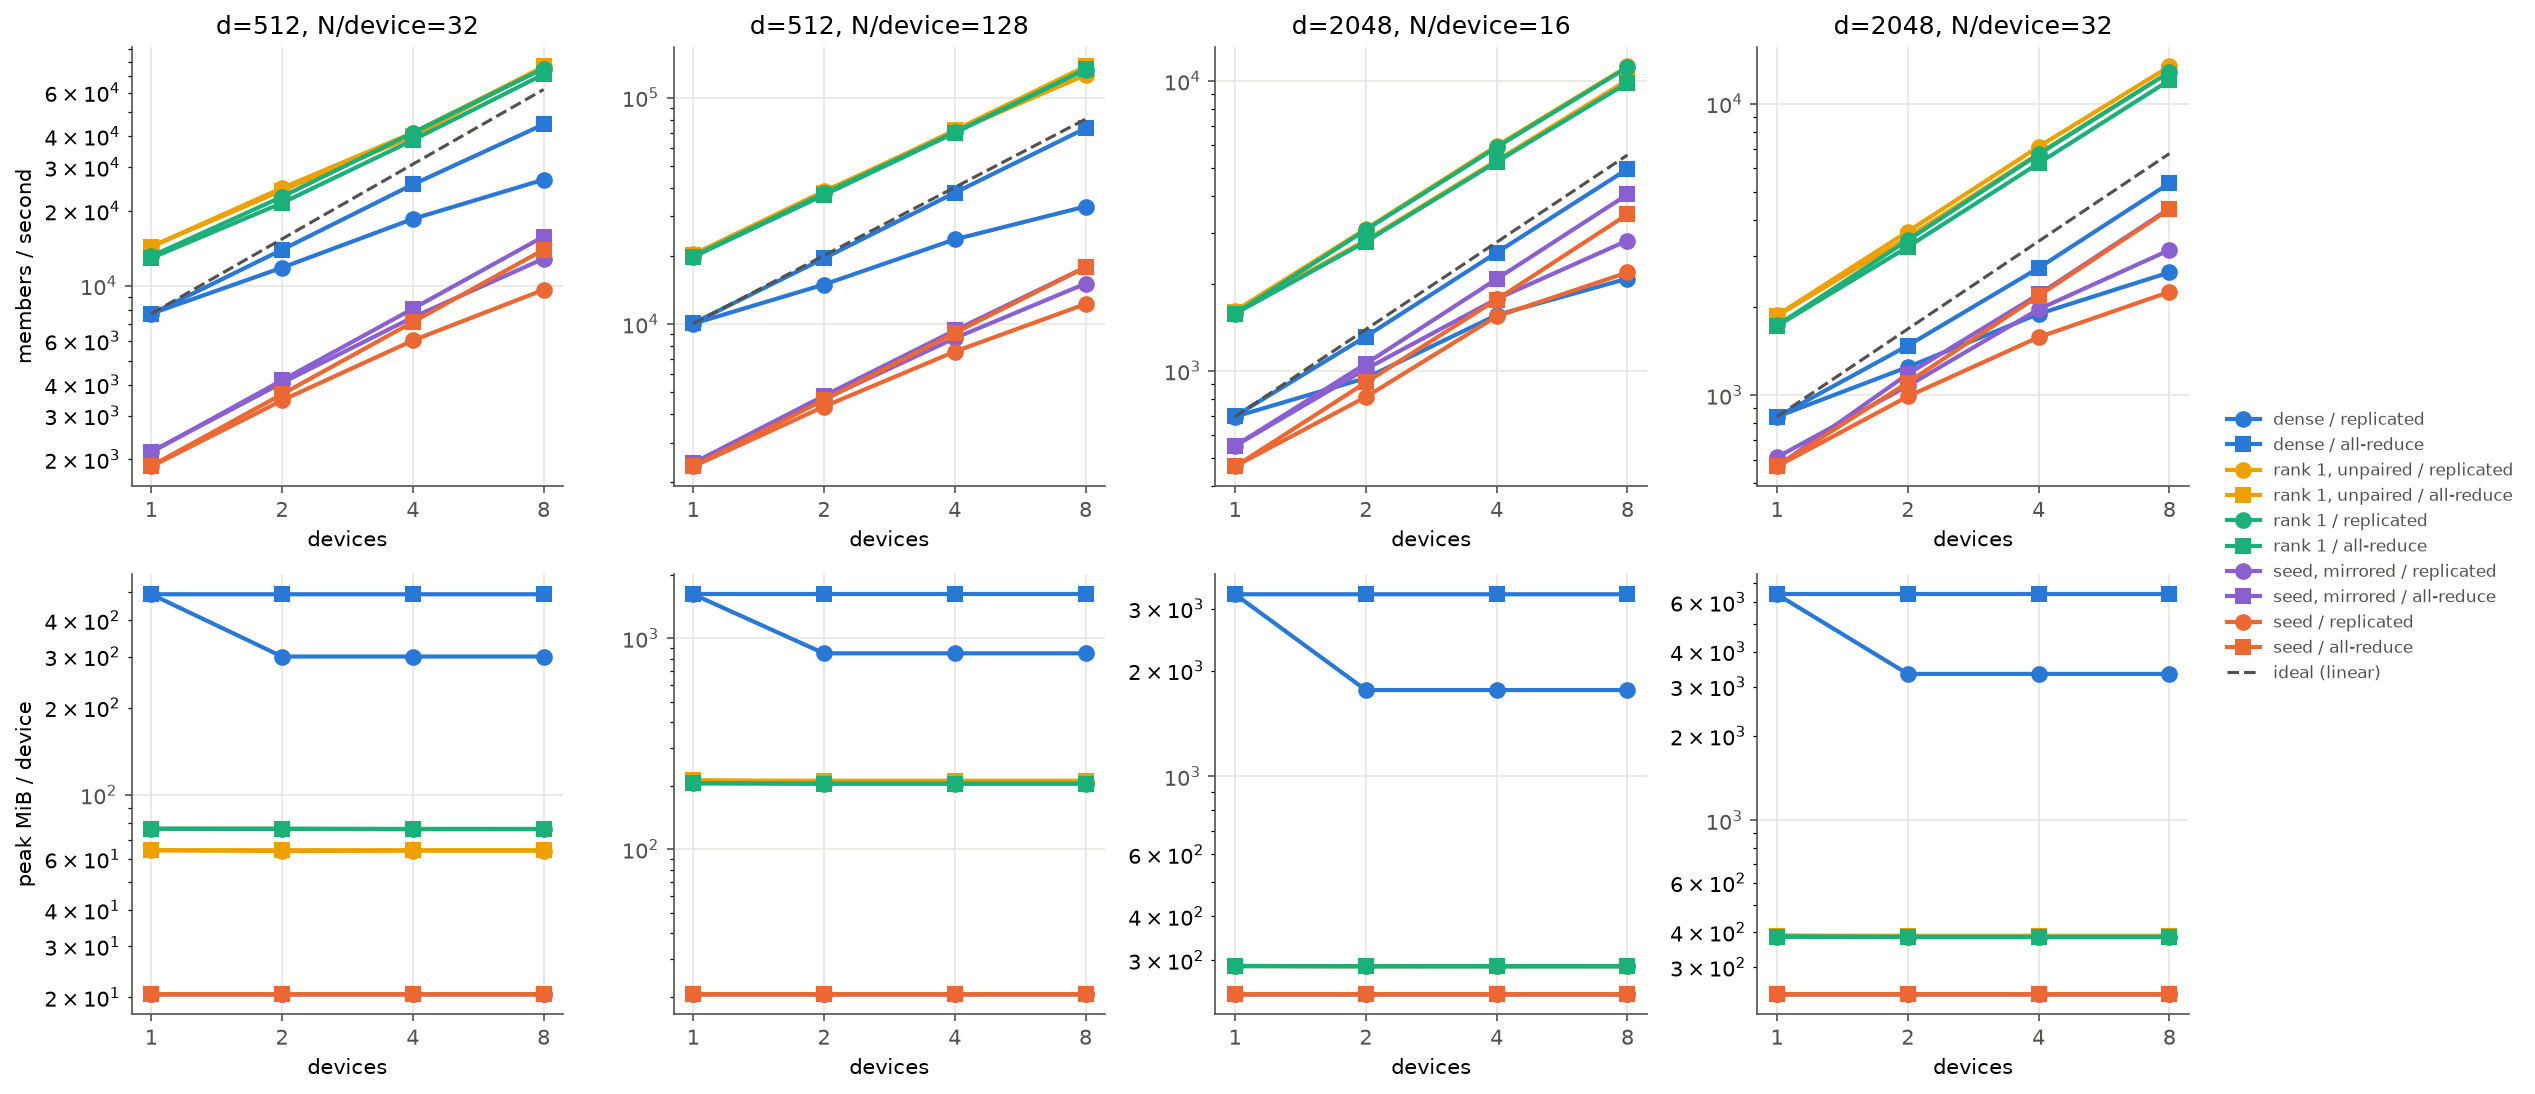
\includegraphics[width=.9\textwidth]{../experiments/phase2/figures/m2-weak-scaling.png}
  \caption{A100 weak scaling: population per device stays fixed. Top: throughput per
    device relative to each series' smallest device count; 1 is ideal. Bottom: peak
    memory per device. A flat memory curve means adding devices does not increase that
    variant's per-device memory requirement at the stated population per device.}
  \label{fig:m2-a100}
\end{figure*}
\begin{figure*}[p]
  \centering
  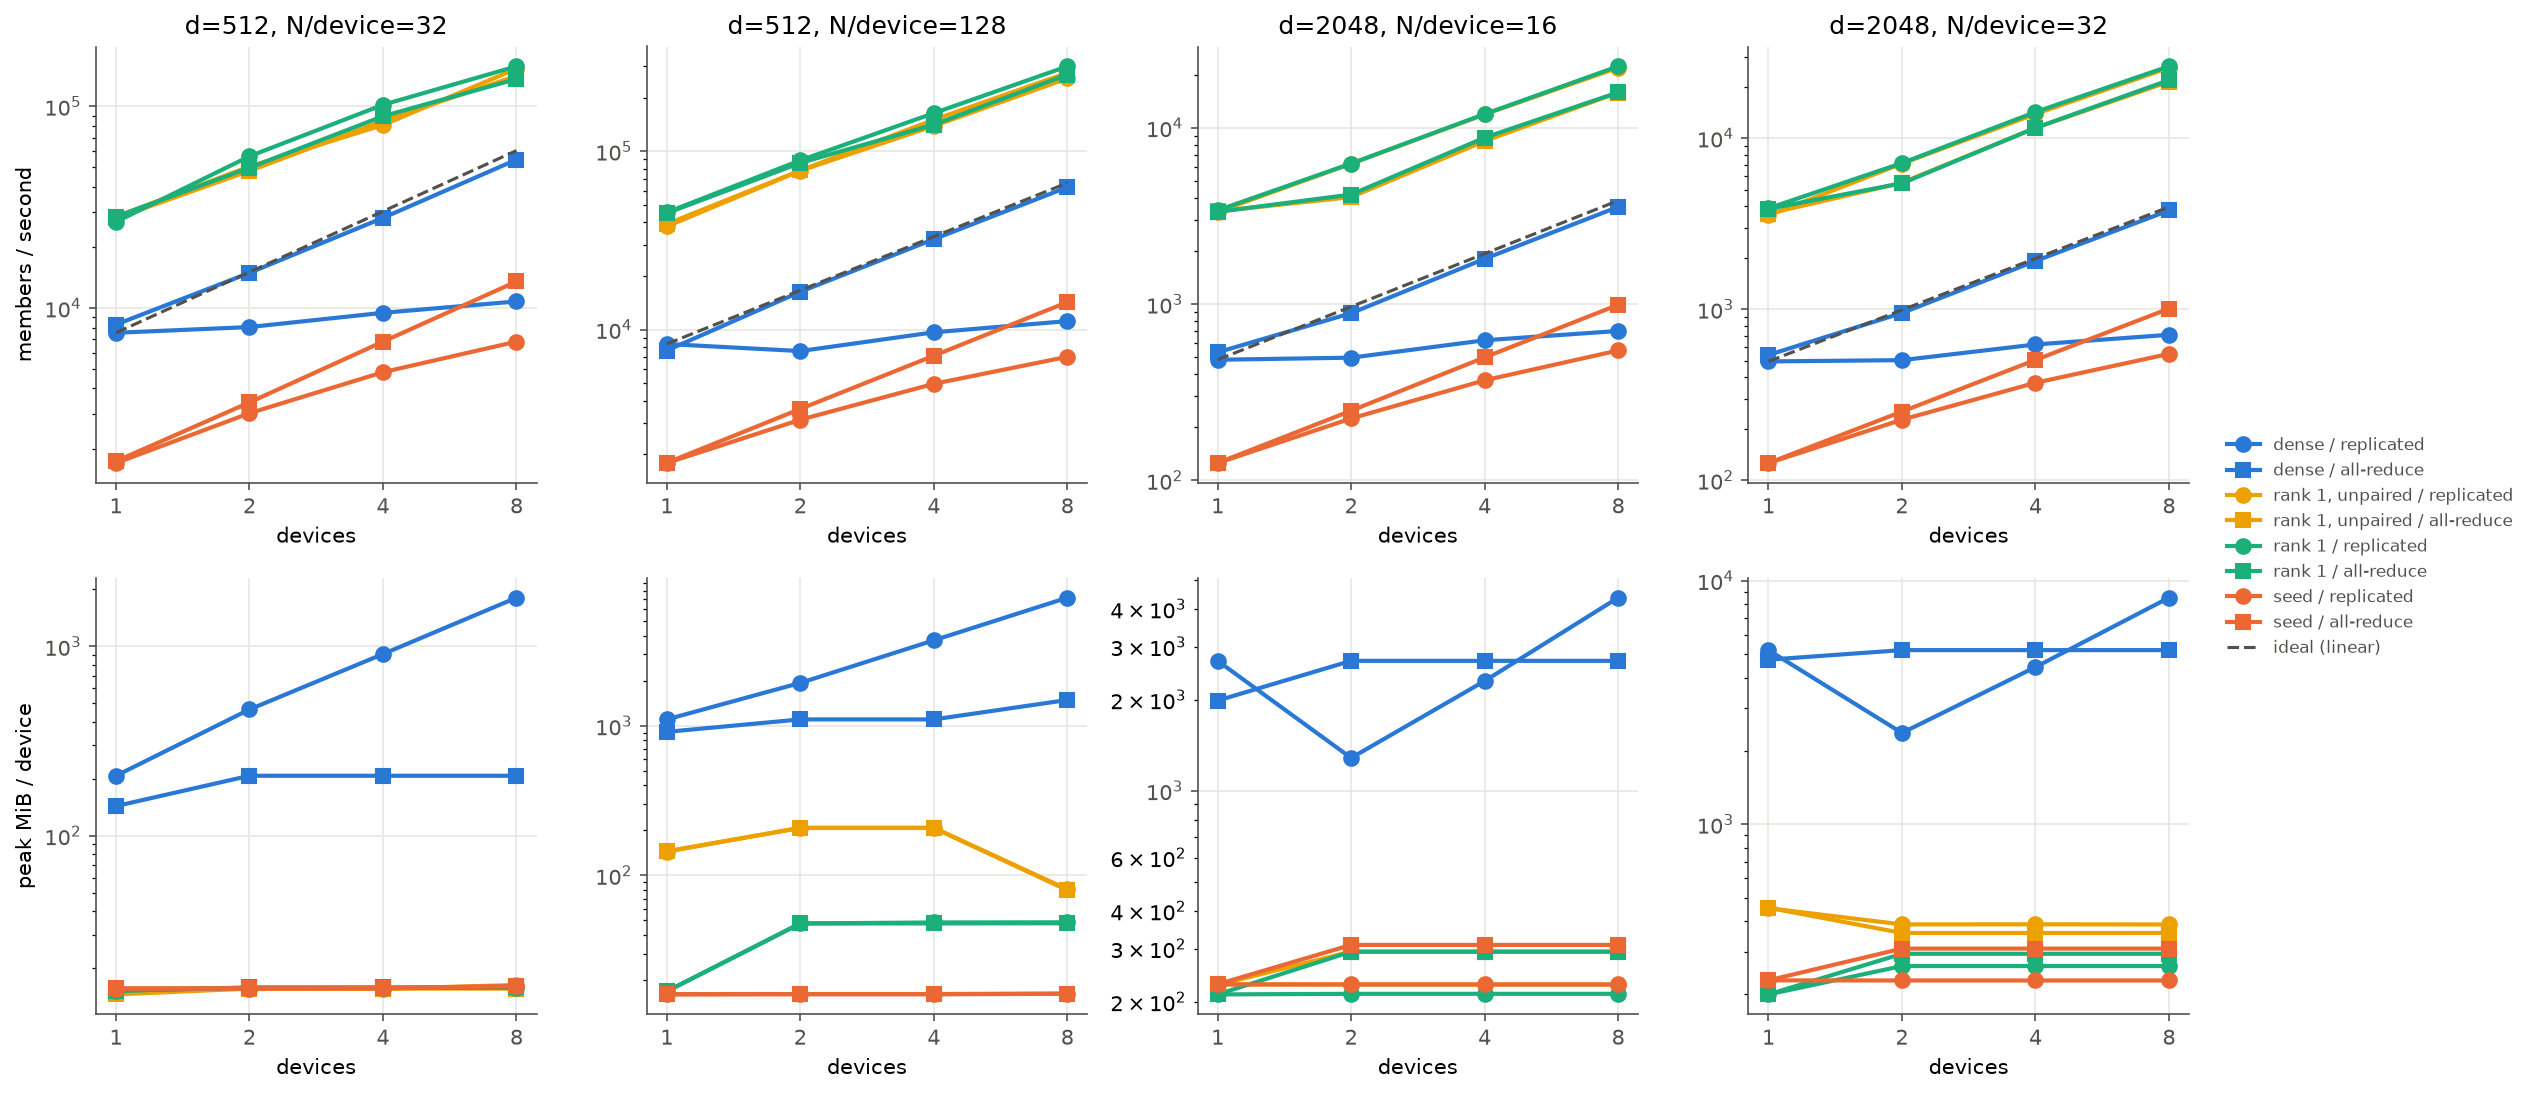
\includegraphics[width=.9\textwidth]{../experiments/phase2/figures-tpu-v5e8/m2-weak-scaling.png}
  \caption{TPU weak scaling at fixed population per device: relative throughput per
    device (top) and peak memory (bottom). Replicated dense reconstruction has the
    largest efficiency loss and its memory grows with the total population.}
  \label{fig:m2-tpu}
\end{figure*}


\section{Reproduction}
\label{sec:repro}

The measurement figures and tables regenerate from scripts and saved results in the
experiments' repository. Each results directory's README records the session that
produced it, including the platform, code version, environment and incidents. The library
is released publicly \librarycite{}; the experiments and manuscript are at \paperurl{}.

In \texttt{experiments/phase2}, \texttt{plot\_paper.py} generates the block-placement
plot, \texttt{plot\_cost.py} the main and appendix cost plots, and \texttt{plot.py}
the scaling grids. In \texttt{experiments/countdown}, \texttt{plot\_e13.py} generates
both the main learning curves and the frozen-embedding comparison;
\texttt{plot\_e19.py} generates the population-16 comparison and \texttt{plot\_e17.py}
the real-model placement plot. The synthetic-alignment plot comes from
\texttt{experiments/phase0/plot.py}.

\texttt{make -C paper} runs the table generators and the revised figure generators,
then builds the PDF. \texttt{paper/Makefile} lists the commands, and
\texttt{paper/README.md} explains how to select the Python environment. Each table
generator accepts \texttt{--latex} and writes the file included in the manuscript;
generated tables are not edited by hand.

The worked example, model comparisons, matched-precision check, bandwidth thresholds
and training displacement ranges are reproduced by \texttt{phase2/paper\_evidence.py}.
The timing ranges are printed by \texttt{phase2/timemodel.py}, the overlap bound by
\texttt{phase2/overlap\_bound.py}, and the compiled-program byte counts by
\texttt{phase2/comms.py} and \texttt{phase2/tb2.py}. The library's device-count
invariance test runs on CPU with eight simulated devices. Continuous integration checks
that regenerating tables changes no bytes and that every commit cited by a result record
remains available.
